\chapter{Software Development} % application?
\label{ch:swdev}

	% Brief description and scope for this chapter	
	\section{Introduction}
	\label{sec:sw-intro}

	\begin{comment}
		Microestado del arte:
		Desarrollo para dispositivos android, paradigma particular, no estamos formados en él (y esto ha dado problemas), 
arquitecturas muy particulares, en el momento de comenzar el desarrollo documentación buena pero muy técnica, más para consulta que para formación. Versiones de android para usb host, … => impone requisitos al dispositivo tablet
    (Posibilidad de hilos destruidos en cada momento, atender al giro de pantalla, destrucción de la actividad, …)
    Limitaciones de android como plataforma (java vm, opengl, …)
    Aplicación iphone: funcionalidad limitada, captura de requisitos comenzó por ella, crear un producto a partir del prototipo.
    Se añadió feedback de los médicos con que trabaja Fran en Murcia (Preguntar a Recas) (en particular los logs!)

	\end{comment}

	% Introduction: app + feedback medical staff (hey, it's an important project!)
	The development of a software ECG display application targeted at Android Operating System for mobile devices is the counter-part to the hardware research part of the project.
	This application is to substitute the already developed one for iOS devices, adding funcionality extracted from feedback obtained for that and including extra features which could not be implemented in it. The software must provide functionality to visualize ECG data from Bluetooth or 802.15.4 sources (the latter obtained via the 802.15.4 USB receiver developed in the hardware part of this project) in real-time, as well as to save that data into file logs for afterwards reading.\\

	% Android general
	Android as a development platform provides a wide set of high abstraction level tools to emphasize robust and reusable design for low resource based, quick development cycles. Such benefits require the adequation of the software design and architecture to the constrains imposed by the Android development framework.\\

	% None android formation + android peculiarities
	Given that none of the project team members had received any instruction on this framework, engaging the development of an Android application implies an important risk. Moreover, after the research and training steps concluded, follow up of such risk can not be halted, as the quick, robust software development is only assured when building an standard Android application; dynamic, soft real-time functionality implementation is not discouraged, but also not guaranteed to work.
	Mobile devices development restrictions and common practices are also unknown to the team at the beginning of the project.\\

	% Android limitations
	Even when the aforementioned eased development features are applicable, mobile devices are harsh software environments due to, amongst others, memory and battery constrains, where processes have to handle being suspended by an incoming call or similar external events. This factors are specially critical for an application as the one developed in this project, which needs to continually parse and log data.\\

	% App linked to hw development and a useful tool
	The application is also intended to act as a quick testing front-end for the prototypes produced by the parallel-conducted hardware research. By providing fully-functional application modules since early stages of development, hardware prototypes could be best-case and worst-case checked by directly connecting them to the Android device for data visualization. Throughout the project process, visual verification has proven to be a very effective method when working with large quantities of data which were more easily checked against their visual representation than value-by-value reading.\\

	% Development process
	These factors lead to the adoption of an agile software development process focusing on functionality building while prototyping more high risk involving features. To avoid typical drawbacks of such methodologies, great emphasis is put on the application of characteristics found in \textit{Iterative and Incremental processes}, namely, use case driven and risk focused development. That way, project scheduling is done addressing higher risks first while assuring expected functionality to be implemented on time thanks to the use case model.\\

	\section{Overview}
	\label{sec:sw-oview}
	% Conclusion and chapter presentation
	In the following sections a complete view of the software development project is presented, beginning with the requirements captured for the project and a comprehensive description of the risk analysis process. The use case scenarios identified from the requisites will be detailed next, followed by an explanation of the system design and architecture. Then, the development process will be exposed in an exhaustive manner, and the chapter will finish with a review of the software development project.

	\begin{comment}
	Full implementation, architectural and yadda yadda are presented in Annex X
	\end{comment}

	\section{Requirements}
	\label{sec:sw-reqs}
		% Requirement capture process explanation (also introduction to this section)
		The requirement capture process for the project considers three main stake-holders: the project directors, the EPFL and the UCM as the base project developer parties and the project team members; and is done in two sessions. The first one produces the basic requirement list which describes the system and is used to schedule the earlier development iterations. This is so because of the strong time restrictions this software development project had to cope with. 
		When the critical functionality is achieved and the hardware research reaches a suitable state, the second requirement capture session is conducted. By then, the EPFL and UCM representative had shown the state of the development to the stakeholder party of him, and collected feedback. Thus, the requirements produced by this second session are of a more user-oriented nature.\\

		% ¿Explicar qué intereses tiene cada uno?
		
		% Y ahora, esto:
		The functional and non-functional requirement lists are presented next.

		\subsection{Functional Requirements}
		\begin{itemize}
		\item R01 - Receive raw data via Bluetooth
		\item R02 - Receive raw data via 802.15.4
		\item R03 - Receive raw data from a log file
		\item R04 - Parse raw data into processed data
		\item R05 - Display processed data
		\item R06 - Log raw data
		\item R07 - Log processed data	% Delete if not developed
		\item R08 - Scale View Vertically
		\item R09 - Scroll View Vertically
		\item R10 - Scroll View Horizontally
		\end{itemize}

	% ?Non-functional requirements?
	% 30fps
	% USB-host Android 3.1

		\subsection{Non-functional Requirements}

		The following non-functional requirements are identified:
		\begin{itemize}
			\item The application must display ECG data at 30fps.
			\item The application must run on a Motorola Xoom device.
		\end{itemize}

	\section{Risk Analysis}
	\label{sec:sw-risks}

		Being the project mainly a hardware research project, and considering the software development part of it useless without successful results on the hardware part, a detailed process of risk analysis is mandatory to be conducted since the earlier stages of planning and development so as to avoid wasting manpower on futile work.\\

		The risk list at the end of the project is as follows:
		\begin{itemize}
		\item \textbf{PR1.} Functionality of the application is inferior to that featured by existing iOS application

		\item \textbf{HR1.} 802.15.4 receiver device delayed
		\item \textbf{HR2.} 802.15.4 receiver device unfeasible

		\item \textbf{MR1.} Mobile device unsuitable for target functionality

		\item \textbf{AR1.} Lack of instruction on Android development delays workflow
		\item \textbf{AR2.} Android providing subpar performance when handling required data
		\item \textbf{AR3.} Android rendering capabilities unable to handle required data
		\end{itemize}

		% Risk anaylisis process explanation (decisions, ...)
		This risk analysis focuses on two main risk sources: the parallel-conducted hardware research, and Android as a development platform. Project definition and team related risks are also considered.\\

		The hardware research part of the project delivers the highest probability and impact rated risks. It is so because those risks are external to the software development project scope and thus can not be handled by any of the tools provided by any development methodology. At the same time, should such risks come to be, the impact on the software product would be, in most of cases, as catastrophic as turning the whole development useless thus causing its cancellation.\\
		
		Regarding Android development only a subset of the final set of risks is assessed at first. Every risk in this subset dealt with the team lack of knowledge about the Android platform and was scheduled to be addressed foremost. A last risk is added to this group after the first research on mobile devices limitations regarding potential unfitness of such devices for near real-time display and handling of not-so-small data packages. That risk handling plan proves to be key to the successful outcome of the project as the remaining subset of Android-related risks are linked to Android applications display performance.\\ % Further explanation on this last set?

		The usual project definition and personal risks such as incorrect deadline scheduling or unability to reach critical milestones on time are also pondered, increasing their impact rates as the application would be needed by the hardware device to secure a successful outcome for the project.\\
		
		% Risk Table including evolution
		A detailed view of each assessed risk is provided next, including risk evolution throughout the project lifetime.\\

		% PR1
		\paragraph{PR1.}Functionality of the application is inferior to that featured by existing iOS application\\
		\textbf{Probability:} Moderate\\
		\textbf{Impact:} Very High\\
		\textbf{Description:} Failure to provide an expanded set of features in the Android application when compared with the iOS application renders the software part of the project invalid on its own. It could, then, only be valid as demo software for USB receiver device showcasing. If the device is not finished, then the whole software development project will have been futile.
		The key marker for this risk is unability to generate valid software modules throughout the development that provide required functionality. Failure to reach milestones and use case realizations on time is other important marker.
		Preventive measures are taken to avoid the occurence of this risk since the beginning of the development by a functionality building focused project scheduling for the first development phases.\\
		\textbf{This risk is marked as surpassed at the reviewing meeting of Iteration 2 as all key functionality has been implemented, as planned.}

		% HR1
		\paragraph{HR1.}802.15.4 receiver device delayed\\
		\textbf{Probability:} High\\
		\textbf{Impact:} High\\
		\textbf{Description:} Being the production of the 802.15.4 receiver device dependent on the hardware research part of the project a delay on the estimated milestones for that part of the project is likely to occur. Should that happen, hardware research and development will need to be prioritized over this software project. That could lead to big delays in software production.
		To prevent the rising of further problems derived from those potential delays, the software development process must always work with non-solid, ready-to-change deadlines and milestones. Application functionality is to be ranked in order of importance of implementation to be prepared, in case of an unexpectedly big delay, to leave less important functionality out of the scope of the project.
		Markers to be followed up are: unsuccessful output from hardware research (a new branch of the potential technologies tree has to be explored), failure to reach hardware development or research milestones and delays in the acquisition of tools or devices needed for the hardware project.
		Preventive measures considered are: detailed follow up of the hardware research development, reducing the software development team if manpower is needed in the hardware area, and planning asuming delays on component acquisition.\\
		\textbf{HR1 is monitored throughout the whole software development project, and marked as surpassed at the reviewing meeting of Iteration 5.}

		% HR2
		\paragraph{HR2.}802.15.4 receiver device unfeasibe\\
		\textbf{Probability:} Medium\\
		\textbf{Impact:} Critical\\
		\textbf{Description:} Until hardware research results are successfully delivered there is no guarantee of the viability of the 802.15.4 receiver device. This software development project loses most of its value if such device is not developed, as the iOS application already exists. Developing an Android application with an equal feature set is also a valid objective, so this risk does not render the development invalid: the full team will then work on software development, and requirements will be restated to include more final-user oriented functionality and/or features from the \emph{future} set.
		This risk can be monitored with the following markers: unsuccessful output from hardware research and failure to reach hardware development or research milestones. Being both external to this software project, no preventive measures can be applied apart from scheduling allowing smaller team sizes for the software area.\\
		\textbf{The probability of the risk is reduced to low after the reviewing meeting for Iteration 3, when the critical hardware research has concluded with positive results. HR2 is marked as surpassed when the production of a device prototype is finished and tested.}

		% MR1
		\paragraph{MR1.}Mobile device unsuitable for target functionality\\
		\textbf{Probability:} Low\\
		\textbf{Impact:} Critical\\
		\textbf{Description:} Even when mobile devices technical specifications have increased significantly in the previous years, specially regarding CPU power and rendering capabilities, the soft real-time requirements of the project in terms of data manipulation and visual representation involve a low probability risk of the application being unsuitable for such devices. The risk probability is decreased by the fact that similar featured applications exist both for iOS and Android powered devices. Even so, the 802.15.4 receiver device USB interface does not allow for this risk not to be reckoned.
		Preventive measures considered: quick prototyping of critical functionality to discard  unfeasibility, conduction of performance tests, both rendering and data handling related, in the target device and testing of USB-Android communication as soon as possible in the project schedule.\\
		\textbf{As performance tests are conducted on early builds of the application, the need of further research on this risk arises as the data handling performance in the target device is low, but not as low as the rendering performance. Thus, this risk is unfolded into risks AR2 and AR3, both related to Android performance when handling the aforementioned tasks. This risk follow up is then halted, as it is no longer needed.}

		% AR1
		\paragraph{AR1.}Lack of instruction on Android development delays workflow\\
		\textbf{Probability:} High\\
		\textbf{Impact:} Moderate\\
		\textbf{Description:} None of the team members has received any instruction on Android development and throughout research is not viable because of time restrictions. It is reasonable to foresee potential delays in the development because of the parallel instruction-development flow, as well as the need to rewrite parts of the system rendered obsolete when further knowledge is acquired.
		Application malfunctioning, unexpected behaviours and low performance are markers to be tracked.
		As a preventive measure a short instruction time will be scheduled at the beginning of the project, but every team member is responsible to continue his instruction throughout the whole project. Application builds are to be checked for big differences against canon Android applications behaviour.\\
		\textbf{The risk is marked as surpassed after Iteration 3, as critical functionality has already been implemented and tested, though Android instruction is not halted.}

		% AR2
		\paragraph{AR2.}Android providing subpar performance when handling required data\\
		\textbf{Probability:} Moderate\\
		\textbf{Impact:} High\\
		\textbf{Description:} The benefits of the high-level, single application model provided by Android are such in behalf of the sacrifice of performance. In this project soft real-time requirements are present, and the system needs to process around 250 ECG wave samples \cite{ecg.del.paper} (among other data) per second. Android code reutilization and class based programming suggested practices, the absence of an explicit memory management API and the employment of the Garbage Collector only complicate the achievement of such requirements.  
		Special care will need to be put on the development and performance checks are to be conducted regularly on generated builds to ensure the avoidance of this risk.
		If evidence is found of Android inability to provide the required perfomance (and there is no way of attributing the failure to the team's lack of ability), low-level Android development will be considered. As the probability of this last scenario to occur is quite low, no research will be conducted in low-level Android development until mandatory.\\
		\textbf{The risk is verified to be happening during Iteration 2 testing phase. Lack of care on memory management is found to be the problem, and is solved in Iteration 3. The risk is marked as surpassed after the review meeting for Iteration 4.}

		% AR3
		\paragraph{AR3.}Android rendering capabilities unable to handle required data\\
		\textbf{Probability:} Low\\
		\textbf{Impact:} High\\
		\textbf{Description:} The Android Operating System runs on quite a wide range of devices, each with its own technical specifications. Providing the single application development model that Android features requires many software layers, many of them of high abstaction level. The risk exists, thus, that the rendering required by the project could not be achieved within the involved time restrictions. The target device for the project is fixed (see \autoref{sec:sw-reqs} Non-functional Requirements Subsection) as a Motorola Xoom. This device employs a dedicated Tegra2 GPU \cite{xoomspecs} which should suffice, so risk probability is chosen as \emph{low}. Performance tests in the display module are to be conducted, though, so as to make sure that a correct usage of the available resources is being done. 
		If low rendering performance is detected, Android native level rendering API, Renderscript, is to be looked into as a remedy, once the code is assured to be optimized.
		\\
		\textbf{Risk probability is increased to \emph{Moderate} during Iteration 3 as low performance is detected but is considered not critical enough to apply the Renderscript solution. The risk is marked as surpassed in the reviewing meeting of Iteration 4.}\\

		% Conclusion
		Thanks to this risk analysis the project schedule is developed in such a manner that it prioritizes risk suppressing and the decision is made to plan only the first two of the five intended development iterations, leaving the other three as drafts to allow them to evolve at par with the uncancelled risks.
		Use case realization order is also selected based on this risk analysis, ensuring that higher risk involving features are developed (or at least prototyped) as early as possible.\\
		
		Use cases for the project are presented next, followed by the system architecture description, to allow a finer understanding of the software development project schedule and related decisions, which will be detailed in the next section.
	
	\section{Use Cases}
	\label{sec:sw-ucases}

		The project use cases are now presented following the \emph{use case common style} described by Martin Fowler [Fowler, 2004], as the relaxed template allows for quicker document producing than more detailed descriptions such as those presented by Cockburn [Cockburn, 2001].\\

		Actor listing is omitted in all the descriptions, because of the following implicits:
		\begin{itemize}
			\item The main actor for the use case is the user
			\item The only other actor is the data emitter node, when applicable. It can refer to the Bluetooth emitter device or the USB 802.15.4 receiver device.
		\end{itemize}
		Please note that the 802.15.4 emitter node is not considered an actor as the communication with such device is handled by the USB 802.15.4 receiver, which actually is the considered actor.

		\subsection{UC1. View data from Bluetooth}

			\paragraph{Description} The user wish to receive and visualize data from a Bluetooth ECG node in real-time. He will start the communication, visualize real-time received data and finish the connection once done.\\
			\\This use case captures requisites R01, R04, R05, R06, and R07.

			\paragraph{Preconditions} The application is in the main menu screen.
			\paragraph{Main flow}
				\begin{enumerate}
				\item User indicates his will to start Bluetooth data visualization.
				\item The system prompts for the node to connect to.
				\item User specifies the desired node.
				\item The system manages connection to the node. If unable to establish the connection, see AF1.
				\item The Bluetooth node sends data to the system.
				\item The system shows processed data to the user. Received data is also logged.
				\item The user can now adjust view parameters (See UC4)
				\item User chooses to finish data visualization.
				\item The system closes active connections and stops data visualization.
				\item The system returns to the main menu.
				\end{enumerate}

			\paragraph{Alternative Flow 1} The system cannot establish connection to the Bluetooth node selected by the user.
				\begin{enumerate}
				\item The system notifies the user about the problem.
				\item The system returns to the main menu.
				\end{enumerate}

		\subsection{UC2. View data from USB Receiver}

			\paragraph{Description} The user wish to receive and visualize data from 	an 802.15.4 ECG node in real-time. He will start the communication, visualize real-time received data and finish the connection once done. The data from the node will be received via the USB 802.15.4 receiver device.\\
			\\This use case captures requisites R02, R04, R05, R06, and R07.

			\paragraph{Preconditions} The application is in the main menu screen.
			\paragraph{Main flow}
				\begin{enumerate}
				\item User indicates his will to start USB receiver data visualization.
				\item The system asks the user to connect the USB receiver.
				\item User connects the USB receiver.
				\item The system manages connection to the USB receiver. If unable to establish the connection, see AF1.
				\item The USB receiver device sends data to the system.
				\item The system shows processed data to the user. Received data is also logged.
				\item User can now adjust view parameters (See UC4)
				\item User chooses to finish data visualization.
				\item The system closes active connections and stops data visualization.
				\item The system returns to the main menu.
				\end{enumerate}

			\paragraph{Alternative Flow 1} The system cannot establish connection to the USB receiver device.
				\begin{enumerate}
				\item The system notifies the user about the problem.
				\item The system returns to the main menu.
				\end{enumerate}

		\subsection{UC3. View data from log file}

			\paragraph{Description} The user wishes to read a log file created from a real-time visualization session. He will specify the log file to load, visualize stored data and finish visualization once done.\\
			\\This use case captures requisites R03, R04 and R05.

			\paragraph{Preconditions} The application is in the main menu screen.
			\paragraph{Main flow}
				\begin{enumerate}
				\item User indicates his will to start log data visualization.
				\item The system prompts for the log file to load.
				\item User specifies the desired file.
				\item The system reads the selected log file.
				\item The system shows logged data to the user.
				\item User can now adjust view parameters (See UC4)
				\item User chooses to finish data visualization.
				\item The system stops data visualization.
				\item The system returns to the file selection menu.
				\item User selects to return to main menu. Else follow from step 3.
				\item The system returns to the main menu.
				\end{enumerate}

		\subsection{UC4. Adjust view parameters}

			\paragraph{Description} When visualizing ECG data the user wishes to adjust view parameters such as plot vertical scale, plot vertical scroll and plot horizontal scroll.\\
			\\This use case captures requisites R08, R09, R10.

			\paragraph{Preconditions} The application is displaying ECG data.
			\paragraph{Main flow}
				\begin{enumerate}
				\item User indicates his will to change the vertical scale.
				\item The system updates plot vertical scale.
				\item User indicates his will to change plot vertical scroll.
				\item The system updates plot vertical scroll.
				\item If the displayed data is read from a log file, see AF1.
				\end{enumerate}
			
			\paragraph{Alternate Flow 1} The user is able to control horizontal scroll parameter.	
				\begin{enumerate}
				\item User indicates his will to change the horizontal scroll.
				\item The system updates plot horizontal scroll.
				\end{enumerate}

	\section{Design and Architecture}
	\label{sec:sw-arch}
	

		\begin{comment}
		Design made targeting easy expansion of the code.
		Android development framework imposes the utilization of a derivate of the Activity class as the entry point for the application. The idea is that an application is composed of various Activities, providing each of them a screen with which users can interact in order to do something \cite{andev-activity}. 
		\end{comment}

		The design of the software application is done targeting easy extension of the functionality which allows an incremental realization of the identified use cases and quick, isolated prototyping of new features in a manner in which already developed ones are not afected.\\

		The Android Software Development Kit being the base technology employed in the development, the Android Application Framework conditions the basic architecture of the system. Particularly this framework imposes the utilization of a derivate of the Activity class as the entry point for the application. The idea is that an application is composed of various Activities, providing each of them ``a screen with which users can interact in order to do something'' \cite{andev-activity}.\\

		The correct usage of the activities model in the Android framework includes declaration of them in the application manifest (see \cite{andev-activity} for reference) and a number of other steps which are excessively formal for the target comfort and speed-of-operation levels regarding development of extensions. Specifically the application gives support for a number of data sources, namely Bluetooth, log file and USB device, each one with its own needs in terms of user interfaces and interaction. Moreover, new data sources would possibly require different interfaces than those already developed.\\

		In such an scenario the decision is made for the architecture of the application to override Android activities model, employing only a single Activity which will implement a stack of user interfaces each with its own logic and behaviour, in the same manner Android does with the activities but allowing more flexible development. The inclusion of a new interface or set of interfaces is, thus, simplified, and every application entity is given the ability to present its own menu to the user. This is specially useful when including new data sources with special interface requirements to the application.\\

		An overview of the application architecture is presented in \autoref{fig:arch-global}.

		\begin{figure}[h]
		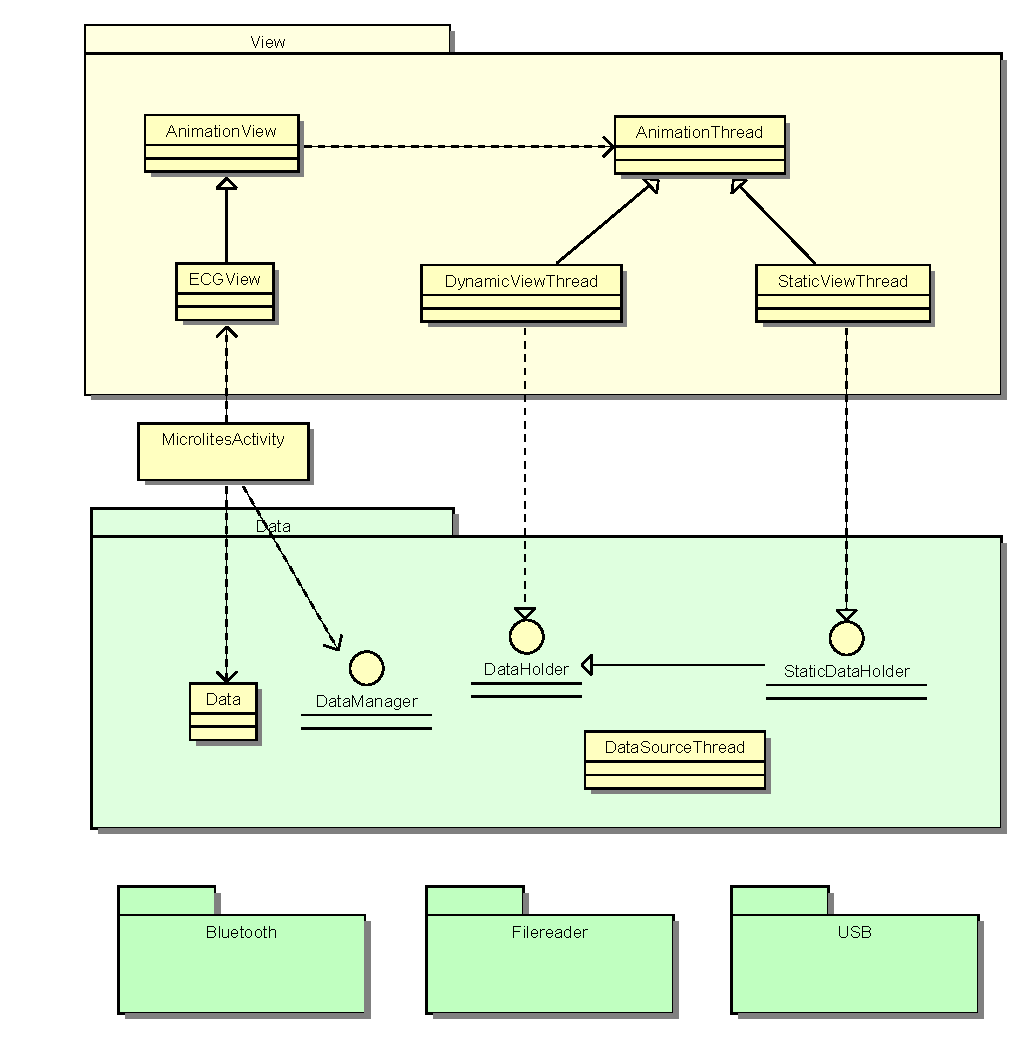
\includegraphics[scale=0.75]{mlts-arch-main}
		\centering
		\caption{Architecture overview}
		\label{fig:arch-global}
		\end{figure}

		At the core level the main Activity, the View package and the Data package are present, as well as three packages (Bluetooth, Filereader, USB) which will be dealt with later. These components provide the basic elements which compose the model over which actual functionality is built, and are to be seen as the tools available for the overlaying software layer which is addressed next.\\

		The main Activity of the application assumes the role of the central coordinator and is responsible for creation and management of area specific managers, application level data and handling of the aforementioned user interfaces stack. It is also responsible, as the entry point of the application, of the presentation and behaviour management of the main application menu which gives access to actual functionality, delegating in the specific managers.\\
		
		Of all those tasks, the most important are the initialization and eventual finalization of data visualization flows in collaboration with the appropiate area specific manager. Throughout the process, mainly controlled by the activity, components required for the visualization process are initialized, delegating area specific tasks to the manager. Eventually, the manager assumes the control of the application flow, leaving the activity as a dispatcher of input events.\\

		% Model: Core, domain specific components that require realization in order to work.
		% Model involves: a Manager, a DataSource and a DataHolder (as well as a DataParser) and, if visualization is required, the ECGView and a ViewThread derivate.
		% The model needs to be realized for it to work, the Activity is just an engine running an instance of the model.
		% "It follows a factory pattern, but the factory is the Activity."

		These managers are part of the so-called, in the project terminology, a model; and the activity can be portrayed as the model manager. Conceptually a model is a set of software entities which live in the application and handle the data flow from a given data source towards a data holder, including or not, the visualization of such data. A model contains a Manager which is the entity responsible of the handling of the rest of the model entities. Please note that this model scheme is  specific to the domain of the project and is not a general one.

		\begin{figure}[h]
		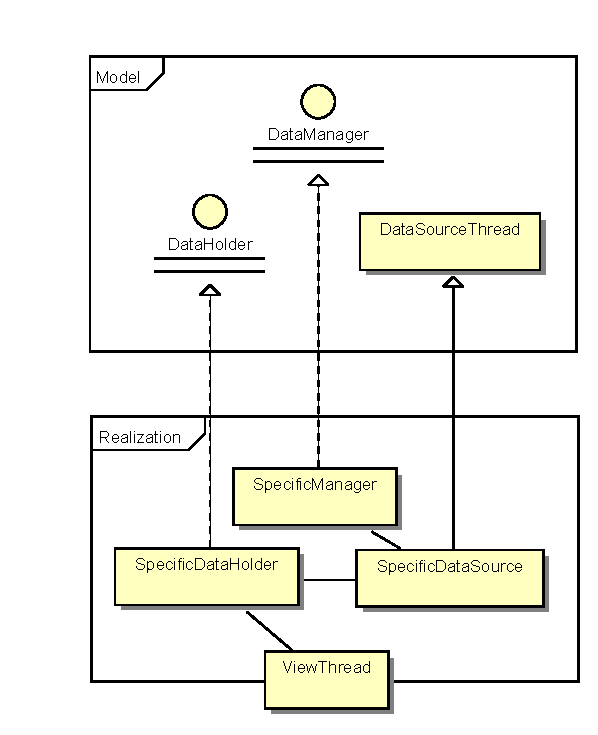
\includegraphics[scale=0.75]{mlts-arch-model}
		\centering
		\caption{Data-flow model realization}
		\label{fig:arch-model}
		\end{figure}

		This conceptual model scheme is provided by a subset of the classes and interfaces shown in \autoref{fig:arch-global}. For actual functionality building a realization of the model is to be developed, giving actual meaning to the scheme. In the scope of the project four model realizations have been implemented and will be detailed later.\\

		A model realization is composed of implementations of the following elements from the core level exposed before: 1) a Manager, which handles user interaction and required preparations; 2) a DataSource that manages raw data obtention from the actual source, and processing and sending of such data to a 3) DataHolder, which stores and handles the data in any required way and, if data visualization is required 4) an implementation of a view thread.\\

		More detailed approaches to all the concepts exposed in this introduction are built throughout the following subsections.

		\subsection{View Package}
		\begin{comment}
		Real-time rendering required a special, non full common functionality (slide, scroll, ...) providing View derivate: SurfaceView. It provides a bitmap surface where you can draw whatever you want. Derived into AnimationView with employment of AnimationThread for obtaning a good old while(!finished) \{update(); render();\} loop.
		That structure derivates into ECGView which is a domain specific specialization of AnimationVeiw and Dynamic- and StaticViewThread. The later two implement behaviour expected of Dynamic and Static data visualization respectively (more on this on the Data Package)
		Programming style in this area closer to C than to an OOP language in order to maximize performance. (Talk about intolerable initial performance caused by extreme number of new each step and too much relaying on GarbageCollector?)
		\end{comment}

		The set of classes encompassed in the View package (see \autoref{fig:arch-global}) provides both a base rendering architecture in an update-render loop style not initially present in the Android framework and the specialization of such architecture for the specific project domain, i.e. plotting of the electrocardiogram wave and its relevant points.\\

		Regarding rendering Android provides a set of common employed visual elements. These implementations try to simplify the developer's work by giving customizable solutions to common scenarios, such as rendering a list of elements or a drop-down selection object, in a visually pleasing way. All these elements are part of the hierarchy of Android's View class, and implement a composite pattern for rich menu-building.

		The soft real-time rendering imposed by the project restrictions requires an specific View \cite{andev-view} class derivate: the SurfaceView. This kind of View provides a bitmap surface where pixel-level rendering is allowed. A set of rendering tools is also provided by Android. The architecture developed on top of that view extends the SurfaceView to an AnimationView and delegates the rendering to an AnimationThread. This last entity is the one providing the update-render loop employed for the real-time rendering. The drawback of employing a SurfaceView as the base is that such element does not provide common employed functionality as scrolling or zooming.\\

		The actual, domain specific rendering functionality providing threads are implemented employing the aforementioned layer as a base. The precise entities are DynamicViewThread and StaticViewThread, and are referred in this document as implementations of the view thread, even if such class does not exist in the project. This two classes implement the required behaviour for dynamic and static data visualization respectively, and obtain the data to be shown from a data source entity. Such entity is dealt with in the following section. The reason for different entities to exist for static and dynamic rendering is also detailed there.\\

		\subsection{Data Management Package}
		\begin{comment}
		Data class acting as a centralized data storage. Provides app-level synchronization too.
		Different models for static and dynamic data management.
		Dynamic: manages its own data and implements replacemente and discard politics, data is provided by single units. This is so because of the way the data is received and then parsed in real-time.
		Static: obtains a reference to the data location, which is where the actual data manipulation is done. This way huge ammounts of data transfering is avoided (read file can contain lots of megabytes of data which can't be passed at once to the holder). First try was passing the whole array of samples but that was unassumable in real-time.
		DataSourceThread is a receiver by concept, but concrete implementations might require actual communication, that is, data reception \emph{and} data sending. As a developer facility, any DataSourceThread must provide an implementation of a method for writing data into the actual raw data source, expected to act in a similar manner to the one the DataSourceThread does in the inside.
		\end{comment}
		
		This package contains data storage and handling related entities. Differentiation between two types of data managed by the application depending on their purpose is mandatory. On one hand is the application level data, which is specific or non-specific information shared by the whole application. On the other hand is the data received from a source that must be visually presented to the user or stored for later visualization. Providing software tools allowing the modelling that data flow is the key task of this package.\\

		The class Data acts as a centralized application level data storage. It is a singleton and is accesible by every entity in the system. It also provides synchronization methods for correct inter-thread communication.\\

		The rest of the entities of the Data package are employed in the aforementioned model scheme, and specify the expected behaviour of each element involved in a data flow. As indicated before, specialization of these entities is required for the realization of the model.\\

		%\begin{wrapfigure}{l}{0.35\textwidth}
		\begin{figure}[h]
		\begin{center}
	    	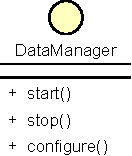
\includegraphics[width=0.20\textwidth]{mlts-ent-datamanager}
  		\end{center}
  		\caption{DataManager interface}
		\end{figure}
		%\end{wrapfigure}


		DataManager is the interface to be implemented by the model controller. It is responsible for the configuring, starting and halting the data flow provided by its controlled entities. It also participates in the process of initialization of the visualization of a data flow by communicating a DataHolder with the respective DataSourceThread.\\

		A DataSourceThread is a thread which provides data to other entities in the system, generally to a DataHolder. It is a specialization of Thread with functionality to start and stop the flow of data. This data is usually received from an external entity, such as a USB device or a file, and concrete implementations  might require an actual communication between the two, forcing the DataSourceThread to send data to the other end of the connection. Because of that, any specialization of this class must also listen to petitions of writing to its data provider when available.\\

		%\begin{wrapfigure}{l}{0.35\textwidth}
		\begin{figure}[h]
		\begin{center}
	    	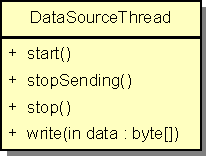
\includegraphics[width=0.3\textwidth]{mlts-ent-datasource}
  		\end{center}
  		\caption{DataSourceThread class}
		\end{figure}
		%\end{wrapfigure}

		The processing of raw data sent by the data providers to the DataSourceThreads is expected to be done in the latter, so the data transferred throughout the application is of a processed nature. To this end the DataParser entity from the Utilities package is available.\\

		The expected receiver of the data sent by a DataSourceThread is a DataHolder. This interface provides domain-specific data handling abstract methods and definitions. An implementation of a DataHolder must handle the reception of ECG wave samples, delineation points, synchronization points and heart-beat-rate values.\\

		%\begin{wrapfigure}{l}{0.35\textwidth}
		\begin{figure}[h]
		\begin{center}
	    	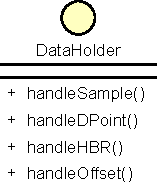
\includegraphics[width=0.20\textwidth]{mlts-ent-dataholder}
  		\end{center}
  		\caption{DataHolder interface}
		\end{figure}
		%\end{wrapfigure}

		The actual way in which that data is employed depends on the concretion of the interface, and might or might not involve visual representation. When visual representation is required, the view thread implementation should also implement the DataHolder interface.\\

		%Dynamic: manages its own data and implements replacemente and discard politics, data is provided by single units. This is so because of the way the data is received and then parsed in real-time.
		%Static: obtains a reference to the data location, which is where the actual data manipulation is done. This way huge ammounts of data transfering is avoided (read file can contain lots of megabytes of data which can't be passed at once to the holder). First try was passing the whole array of samples but that was unassumable in real-time.

		There are two different specifications for the data holders: DataHolder and StaticDataHolder. This is so because of the two modes of operation of the application. One is real-time data visualization and the other is log file visualization. The former is called dynamic visualization and the latter static visualization, and the behaviour of their DataHolders is not the same.\\

		Dynamic visualization represents data received in real-time by the DataSourceThread. The DataSourceThread obtains the data from an external entity, processes it and sends it to the DataHolder. This data usually arrives in groups of variable size, and is provided to the DataHolder in single units once processed. In this scenario the DataHolder is the view thread, and handles data however considers optimal. In the implementations developed in this project a fixed amount of data is held and older information is replaced by the new one as it arrives.\\

		Static visualization, on the other hand, involves reading a file, usually mega-byte sized. The reception of big quantities of data in single units by the data holder, as would occur if  the original DataSource specification was employed, could lead to severe slow-downs and application performance would be affected. To avoid such issues, the StaticDataHolder specification is developed.\\

		A StaticDataHolder does not actually hold the data: it delegates that task to its DataSourceThread. The data source will provide the StaticDataHolder with a reference to the actual data. This way big amounts of data transferring is avoided. The inheritance relation between DataHolder and StaticDataHolder is imposed by the architecture, which requires a DataHolder to be passed to a DataSourceThread.\\

		\subsection{Utilities Package}
		\begin{comment}
		Contains application level reusable components as two different DataParsers (one for real-time, on for static data which does not store what it reads). Also contains the Viewport entity employed as a container of the view parameters. An unused color picker is there (not mention!)
		\end{comment}
		This package contains reusable components providing very specific functionality so they are considered utilities: RealTimeDataParser, StaticDataParser and Viewport.\\

		A data parser is the entity responsible of the processing of the raw data obtained by a DataSource into the domain specific data that the application manages. There are two implementations, one for real-time data reception, RealTimeDataParser, and the other for static data reading, i.e. a log file. The real-time data parser is also responsible of storing the received raw data to a log file.\\

		A data parser is intended to be contained in a DataSourceThread. It receives the bytes of raw data and, upon successful identification of a valid data element, notifies the corresponding DataHolder entity of the arrival. In a theoric, performance-independant model, this behaviour would be incorrect: the data parser would leave the processed data \emph{in} the DataSourceThread, which would then make the transfer of information to the data holder. This kind of implementation is not valid with the soft real-time requirements of the project, as the data source - data parser - data source - data holder flow would be a severe bottle-neck.\\

		The Viewport entity is a container for the visualization area settings. It represents the window in which the data plotting is done, and holds information about size and position of it. It also contains data about the horizontal and vertical scale of the rendering and handles modification of all these parameters. It is employed by the view thread hierarchy.
		
		\subsection{Data Flow Model Realizations}

		Having explained the data flow model scheme and the core level architectural elements employed in its construction, model realizations implemented are detailed next. For each realization, the concretion of each model element will be exposed including particular details of such implementation.

		\subsubsection{Bluetooth Model}
			The Bluetooth model is a real-time visualization targeted data flow where the actual data provider is a Bluetooth node. As visualization is an objective, this model realization employs a DataManager, a DataSource, a DataHolder and a DynamicViewThread; the latter two being implemented in the same entity. An overview of the realization is shown in \autoref{fig:arch-bt}.\\

			\begin{figure}[h]
			\centering
		    	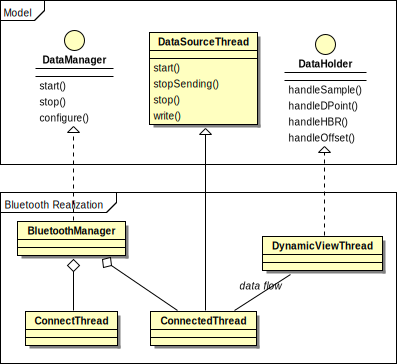
\includegraphics{mlts-arch-bt}
	  		\caption{Bluetooth Model Realization}
			\label{fig:arch-bt}
			\end{figure}

			The specialization of the DataManager is the BluetoothManager. It prompts the user for the device to connect to and handles connection by employing two threads: ConnectThread and ConnectedThread. After discovering the available nodes, it locates the node indicated by the user and launches the ConnectionThread.\\

			This ConnectThread is the thread which actually manages the connection by obtaining its endpoints in the form of a socket. If successful, passes the socket to the manager and finishes its execution. The manager then launches the ConnectedThread, which receives the socket and data flow starts. The reason for employing a thread for establishing the connection is to avoid blocking the application while connecting.\\

			ConnectedThread is the DataSourceThread implementation and contains an entity of DataParser. It receives data sent by the Bluetooth device through the socket, parses it and notifies the DataHolder implementation, which is the DynamicViewThread. The DataParser in DataSourceThread is a RealTimeDataParser and stores the data in a log file while processing.

		\subsubsection{File Reader Model}
			This model realization implements visual representation of ECG data stored in a log file. It is a static view model, in which the user controls what section of the temporal log is shown on-screen, an thus employs an StaticViewThread instead of a dynamic one.\\

			\begin{figure}[h]
			\centering
		    	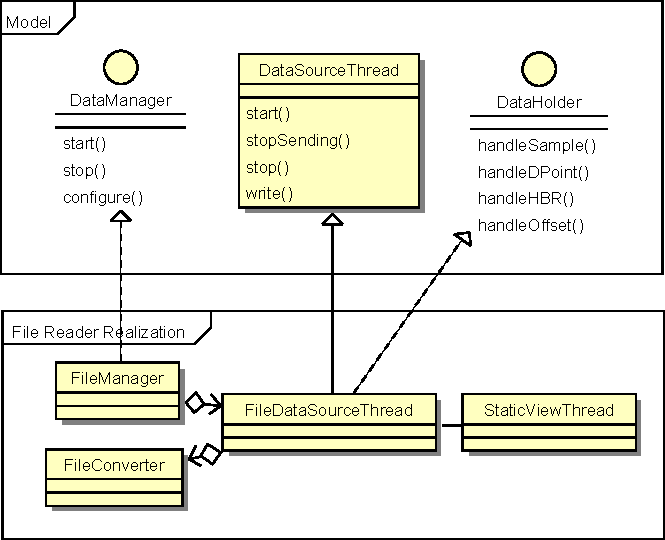
\includegraphics{mlts-arch-log}
	  		\caption{File Reader Model Realization}
			\label{fig:arch-log}
			\end{figure}
		
			The manager in the file reader model is the FileManager class. It presents available log files to the user, handles the selection of one, instantiates the file reading thread and connects this with the view thread. When the user finalizes the visualization of the selected log, the FileManager returns to the log selection menu instead of going directly to the main menu. This is an example of the versatility of the aforementioned view stack scheme, which lets specific managers present as many menus to the user as necessary.\\

			FileDataSourceThread is the thread that reads the chosen file and processes its data. It implements both the DataSource and the DataHolder interfaces, so it acts as the emitter and the receiver of the processed data. The view thread obtains a reference to this same data, thus avoiding big amounts of data transferring in the static view model as explained before. This is an example of the flexibility sought by the architecture design.\\

			The FileDataSourceThread, thus, manages data reading, storage and manipulation. The data is read from files with the aid of the FileConverter entity from this package. This files can be of big size, so they should not be fully loaded onto memory. A partial load is mandatory in such cases, and the next chunk of data is to be read when the ``visualization window'' approaches. All this management is done by the FileDataSourceThread.\\

			When the view is controlled by the user, i.e. horizontal scroll, the event is passed directly into this thread from the StaticViewThread. FileDataSourceThread then updates the portion of the data to be shown. The updated information is consulted by the view thread in the next rendering step. That way, were further file reading required, it could be done in a transparent-to-view manner.\\

			Data processing is done employing an instance of StaticDataParser in the FileDataSourceThread.\\

			The FileConverter entity provides functionality to transform a given file to an Stream, ArrayList or array of bytes, the latter being the expected input format for the available data parsers.

		\subsubsection{USB Model}
			The USB model manages data reception from an USB device and eventual visual representation for the user. It is a real-time data flow, and thus employs a dynamic view thread. An overview of the model is shown in \autoref{fig:arch-usb}.\\

			\begin{figure}[h]
			\centering
		    	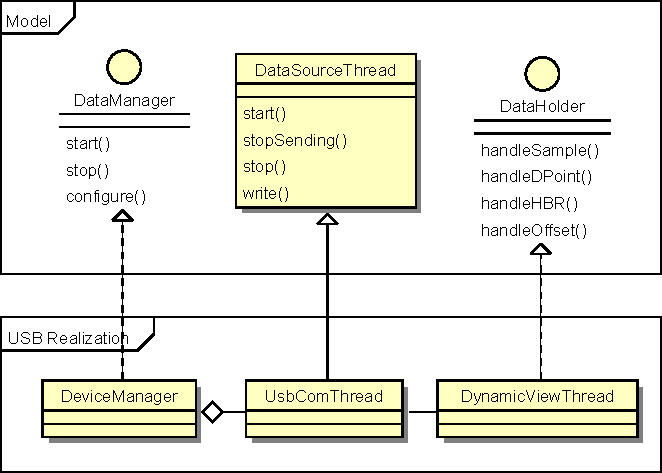
\includegraphics{mlts-arch-usb}
	  		\caption{USB Model Realization}
			\label{fig:arch-usb}
			\end{figure}

			DeviceManager is the realization of the Manager of the model. This entity handles connected USB devices enumeration and selection by the user. If only one device is available, connection is directly stablished with it. Differing from the Bluetooth realization implementation, the actual connection to the device is handled by the DeviceManager in a blocking manner. It is so because USB connection resolution takes very little time and the delay is virtually imperceptible for the user.\\

			Once the connection is stablished, the DeviceManager launches an instance of UsbComThread. This thread is the specialization of DataSourceThread and obtains the raw data from the USB device, processes it employing an instance of DynamicDataParser and sends the results to the view thread. This is a DynamicViewThread entity.

		\begin{comment}
		\subsection{More things (which I don't know where to include}
			
			\texttt{(These with sequence diagrams and all)}
			Explanation of the visualization initialization procedure, as well as the finalization one.
			Example of a full data flow (e.g. bluetooth)
		\end{comment}

	\section{Development Process}
	\label{sec:sw-process}

		\begin{comment}
			Potential iterations
			It1. Bluetooth + Architecture prototype
			It2. USB + Log
			It3. Architecture rewriting
			It4. Adding it all and finishing

			For iteration description:
				+ objectives
				+ objectives description
					realization, done?
				+ Use Cases realized
				+ expected and spent time
				+ extra objectives
				+ prologue to next iteration

			Describe risk statuses updates in each iteration?
		\end{comment}

		% Intro
		In this section a detailed description of the development is presented. The evolution of the application architecture and functionality; design, architectural and implementation decisions and explanations of the circumstances in which they were made, as well as the development of the project schedule are exposed in chronological order.\\

		The section is arranged following the five iterations of the project, developing each one by presenting the target objectives and expected deadlines for the iteration, detailing application evolution with emphasis on use case realization and risk suppressing achievements and demonstrating the state of the project as assessed on the reviewing meeting conducted at the end of the iteration.

		% Scheduling
		\subsection{Project Scheduling}
			
			Before diving into the description of the development process an overview of the project schedule % and the reasons for it to be as open as it is
			is mandatory.\\

			As it was mentioned in the previous sections, an agile software development methodology has been applied to the project, even if artifacts from more ordered and structured methodologies have been employed to avoid losing focus on the critical aspects of the development.\\
	
			Software development project being dependent on parallel-conducted hardware research, project assets, both personal and development resources, being shared with the hardware research having the former higher priority, and the team's lack of formation regarding Android development are some of the factors which lead to the adoption of such a mixed methodology. As they have been already exposed in previous sections, they will not be detailed here.\\ %Consult [X][Y][Z]... for details

			In such an scenario, a fully developed, eight month covering schedule is unfeasible, at least with the imposed time restrictions which does not allow much time to be spent on planning. The decision is then made to plan only the earlier project iterations, assuring critical functionality identified from use case development to be implemented as soon as possible as well as higher threat involving risk suppression to be realized.\\

			Actual software project development begins October 15, 2011, being the final deadline set on June 15, 2012. That deadline can not be pushed any further, so an estimated deadline is set on May 31, 2012, leaving half a month for further work or recovering from delays, and seven and a half months of development time.\\
		
			Time is needed for the hardware research to start providing results, and no work can be done in the meantime on related application parts. Considering also that even in the most optimistic scenarios no actual work with the 802.15.4 USB receiver could be done until mid February, the schedule has to assume that the first four months of software development will need to cover the implementation of most of the features, leaving the rest of the development time for implementing hardware-related requirements, which could not actually be scheduled until hardware research was evaluated.\\

			The adopted schedule deals with the aforementioned facts by proposing five iterations, from October 15 to May 30, complying with the fifteen days reserved for contingencies. The first three iterations have a duration of two months, the third one, of a single month, and the remaining one is fifteen days long.\\

			Having the previously developed iOS application as starting point, and being achieved at least the same feature list of that a critical target of the project, the first two iterations are planned so as to realize \textbf{UC1} and \textbf{UC3} which capture requisites expressing such feature list.\\

			The next iterations are just scrapped as no accurate estimation can be done on the state of the project by those dates. Thus, the third iteration is planned to cover the implementation of the remaining features, namely, communication with the 802.15.4 receiver device, the fourth one reserved for polishing the application and the fifth one left for testing and validation. The fourth iteration is to shrink if objectives are achieved quickly to leave more time for validation.\\

			The scheduled distribution of work for each iteration is as follows:\\

			\begin{tabular}{| c | l | l |} % | l | para el hw
				\hline
				It & Dates & Activity \\ \hline
				1 & Oct 15 - Dec 15 & Application base and Bluetooth module\\ \hline
				2 & Dec 15 - Feb 15 & Log module and initial USB module\\ \hline
				3 & Feb 15 - Apr 15 & Final USB implementation \\ \hline
				4 & Apr 15 - May 15 & Polishing \\ \hline
				5 & May 15 - May 30 & Validation \\ \hline
				- & May 30 - Jun 15 & Reserved \\
				\hline
			\end{tabular}\\\\

			Which can be seen as the following expected use case realization dates:\\

			\begin{tabular}{| c | l | l |} % | l | para el hw
				\hline
				It & Dates & Realized Use Case \\ \hline
				1 & Oct 15 - Dec 15 & UC1, UC4 (first version)\\ \hline
				2 & Dec 15 - Feb 15 & UC3, UC2 (first version)\\ \hline
				3 & Feb 15 - Apr 15 & UC2 (final) \\ \hline
				4 & Apr 15 - May 15 & UC4 (final) \\ \hline
				5 & May 15 - May 30 & Validation \\ \hline
				- & May 30 - Jun 15 & Reserved \\
				\hline
			\end{tabular}\\\\

			Throughout the development, as expected, this schedule has to be adapted as the hardware research advances to assess the arise of difficulties and subsequent changes to its planning. Instead of providing a fixed snapshot of the altered schedule at the end of the project, a detailed description of each iteration is presented next, including modifications to the planning and the motivation for making them.

		\subsection{Iteration 1}

			The main objectives for this first iteration are
			\begin{itemize} 
				\item the instruction of the team on Android development, 
				\item the lay out of an initial version of the application architecture and
				\item the implementation of the Bluetooth receiver module.
			\end{itemize}

			The alloted time for the iteration is of two monts, from October 15 to December 15. During this period the hardware research does not require much resources, so in practical terms the full team is employed in the software project.\\

			In order to minimize risk AR1, the instruction of the team on Android development becomes the key objective for the iteration. Development starts with the implementation of the designed base architecture for the application, so it serves as a powerful learning resource. The notion of that implementation as disposable is not abandoned throughout iteration time and it is always considered as a prototype to evolve or be substituted by a more refined version once the team's knowledge of Android increases.\\

			Having the basic architectural framework developed, implementation of the Bluetooth receiver module begins. Special care is put both on design and implementation, as this functionality has to be ready as soon as posible, and little time will be available for reimplementation further in the development.\\

			Testing of both architecture and Bluetooth module is conducted during the whole iteration, specially in the final weeks, so by the end of the iteration Bluetooth module is validated and expected to be stable until the scheduled architectural redesign.\\

			As the Android formation phase takes less time than expected and hardware research does not allow advancing into next iteration at the time iteration objectives are achieved, an extra implementation effort is put to begin implementation of UC4. Adjust View Parameters.\\

			In the review meeting for the iteration the following conclusions are obtained:
			\begin{itemize}
				\item Basic architecture implementation is done.
				\item Android is confirmed to be a very comfortable development environment even if non-standard functionality is not that easily achieved. Instruction is planned to continue.
				\item Realization of UC1-\emph{View data from Bluetooth} is finished. Related user interface is not final, but it is functional, and is to be updated on further iterations.
				\item Realization of UC4-\emph{Adjust view parameters} is done in relation to Bluetooth visualization. As remaining modules are developed, further work is to be done in this field.
			\end{itemize}

			\begin{comment}
			Results and adaptation of pre-planned it2
			Risk evolution!?
			\end{comment}
			
		\subsection{Iteration 2}

			The main objectives for the second iteration are
			\begin{itemize} 
				\item the development of the USB communication module and
				\item the implementation of the Log visualization module.
			\end{itemize}

			The hardware reserarch having provided successful results regarding the initial prototypes of the USB accessory, the scheduled USB module implementation for this iteration is mantained, but delayed until further testing can be done in the hardware area.
			In that scenario this iteration begins with the implementation of the log visualization module.\\

			Module design and implementation are to change little in following iterations to allow the scheduled architecture rewriting to be realized and trying to minimize the possibility of risk PR1. This situation and the fact that a lot of resources are required in the hardware area makes the achievement of this objective fill most part of the iteration time.\\

			Full expected functionality is implemented, including the remaining features from UC4-Adjust view parameters, but validation testing indicates low performance in log visualization caused by big memory requirements. Effort needs to be put into the other iteration objective, so log visualization is halted at this point, scheduling the development of required optimizations for the next iteration.\\

			Having the USB accessory prototype in an usable state, development of the USB communication module begins. At this point the USB accessory could only operate assuming the role of host in the connection, so the disposability of the module is acknowledged. Nevertheless, this implementation is a must if the project goals are to be achieved, as it serves as first-hand instruction regarding USB development in Android. Moreover, if the hardware project is unable to produce an USB slave accessory, with the developed module the project would not have fully failed. Eventually this development has proven being key for the first tests with the actual target hardware platform.\\

			During the implementation of the USB communication module the log writing is improved, so, except for the aforementioned performance optimizations, the log part of the application is finished.\\

			With the basic interface, disposable architecture and fully functional data flow modules, full application functionality is implemented by the end of the iteration, and in the review meeting the following conclusions are obtained:
			\begin{itemize}
				\item Full functionality has been implemented in the application and the product of this iteration is, as expected, the first prototype of the application.
				\item Realization of UC2-\emph{View data from USB Receiver} is done until hardware research advances. Current implementation can act as the actual version of the use case realization if hardware research is not fulfilled.

				\item Realization of UC3-\emph{View data from file log} is done.
				
				\item Realization of UC4-\emph{Adjust view parameters} is now finished. All required view controls are implemented.

				\item Risk PR1-\emph{Functionality of the application is inferior to that featured by existing iOS application} is marked as surpassed, as key functionality is implemented.
				\item Risk MR1-\emph{Mobile device unsuitable for target functionality} is identified to require further monitorization and is unfolded into risks AR2 and AR3.
				\item Risk AR2-\emph{Android providing subpar performance when handling required data} is confirmed to occur and is to be solved in the next iteration.
			\end{itemize}

			\begin{comment}
			Log writing improved.
			USB module done as USB device, valid for arduino and first msp tests
			Log reading implemented, scrolling and such. Tests results indicate low performance, huge memory requirements.
			With the basic interface, first Prototype with (except usb host == 802.15.4) full functionality implemented. That nice and all. Shown to masters and feedback applied.
			On time ?
			
			Took a loong break here for hardware development
			% Here ends electroiltes
			\end{comment}

		\subsection{Iteration 3}
			% This is microlites
			\begin{comment}
			This is the first just-drafted iteration. Starting from the fully functional prototype, architectural and performance fixes were mandatory. Also, given the positive state of the hw research scheduling was done for the rest of the iterations.

			The main objectives for this third iteration are
			\begin{itemize}
				\item the redesign of the application architecture, 
				\item achievement of required performance in data management and
				\item scheduling of the rest of the project time.
			\end{itemize}

			~(Scheduling seems strange as an objective)~

			Architecture redesigned targeting easy adaptation and versatility inside the scope of the application. Redesigned visualization initialization flow.
			Performance increased significantly and memory usage reduced THROUGHOUTLY in real-time view.
			Fixes in modules according to new architecture.
			Talk about scheduling??
			\end{comment}

			This is the first just-drafted iteration of the original scheduling. Taking the prototype obtained in the previous iteration, architectural redesign and performance optimizations are mandatory. Performance optimizations are  identified to be required in two areas: data management and data rendering. Only data management related optimizations are addressed in this iteration.\\

			Iteration objectives are as follow:
			\begin{itemize} 
				\item redesign of the application architecture, 
				\item achievement of required performance on data management, and
				\item scheduling of the rest of the project time.
			\end{itemize}

			The main lack of the basic architecture of the protoype is that it was implemented to serve as a quick prototyping base for the data flow modules. The instruction and knowledge about the platform and the way of operation obtained in the previous iterations are applied in the new architecture design.\\

			This design is done targeting easy inclusion of new data flow modules allowing them to employ their own user interfaces, while providing core level software entities for building those modules. This process produces the architecture as exposed in \autoref{sec:sw-arch}.\\

			A detailed analysis is conducted on the data management related operations in the application, identifying the ubiquitous application of the object oriented model proposed by Java added to the subpar efficiency of the Garbage Collector as the main cause of performance loss. The alteration of the programming paradigm and the employment of as basic software entities as possible, avoiding continuous object instantiation, e.g. substitute an object containing the four parameters of a wave delineation point, by a more basic structure, like the same four numbers stored independently, prove to be the most effective methods of avoiding low performance.\\

			Following such lines of operation, performance regarding data management is utterly improved in spite of a less developer-friendly programming environment. During this process the data flow modules (Bluetooth, USB and Log Viewer) are also tweaked.\\

			The positive results obtained both in the software and hardware areas allow a solid review of the project schedule. The decision is made to keep the division of the remaining project time in two iterations, leaving the last, fifteen days period for unforeseen difficulties. Of the two iterations, the first is to be devoted to implementation of the USB host communication as hardware project estimates completion of a first prototype halfway the iteration; and the second, and last, iteration is planned to be employed in final testing and validation of the application against hardware prototype.\\

			The following conclusions are obtained from this iteration's reviewing meeting:
			\begin{itemize}
				\item The architecture of the application is finished and validated.
				\item User interface is yet to be final and is to be addressed at the following iteration.
				\item Identified solutions for performance issues are to be applied in the rendering area.
				\item Risk AR1-\emph{Lack of instruction on Android development delays workflow} is marked as surpassed as the team feels comfortable enough with Android development.
				\item Risk AR3-\emph{Android rendering capabilities unable to handle required data} probability is increased to Moderate and is to be addressed in the next iteration.
				\item Risk HR2-\emph{802.15.4 receiver device unfeasibe} probability is reduced to Low as hardware research is providing positive results.
			\end{itemize}

		\subsection{Iteration 4}
			\begin{comment}
			Final implementation iteration. Final performance increasing fixes and user interface implementation, as well as user-friendliness globally increased.

			USB Host here!

			The main objectives for this third iteration were
			\begin{itemize} 
				\item the implementation of USB host communication,
				\item the achievement of required performance in rendering and, 
				\item the implementation of user-friendly interfaces.
			\end{itemize}

			This ends the implementation phase, user-friendlyness could be better but what gives. 
			Performance left 50-50 because it was already ok (30fps not 60fps).
			One iteration left, devoted to testing.
			\end{comment}

			This iteration is scheduled to be the last implementation iteration, and its objectives are:
			\begin{itemize} 
				\item the implementation of USB host communication,
				\item the achievement of required performance in rendering and, 
				\item the implementation of actual user interfaces.
			\end{itemize}

			The USB slave accessory prototype is produced on time by the hardware project, and implementation of the actual USB communication assuming the Android device the host role is done in very short time, leaving room for achievement of the rest of the iteration objectives and following validation.\\

			Employment of the identified working solutions for performance issues in the rendering area does not provide the expected results, and further research is required. The bottle-neck in the rendering process is identified to be the context change required by the rendering tools provided by Android. Meticulous research on Android developer resources provides no other solution than minimizing the number of calls to the rendering methods each step. Emphasis is put to the realization of this task, but to no avail.\\

			The problem is the big amount of data required to be drawn each rendering step. A mechanism is developed to minimize the number of lines drawn by joining similar valued wave points, and the performance is improved, but not at the desired level. Nevertheless further work in this area is postponed as the achieved performance lies in the range required by the non-functional requirements of the project.\\

			Implementation of the actual user interfaces to be employed in the application is addressed next. The design of these has been done throughout the last two iterations. The implementation process takes more time than expected as	Android user interface framework is quite specific, and requires adequation to certain rules that have to be studied beforehand.\\

			The remaining time of the iteration is devoted to testing and validation of the application, which has reached a near final state. Conclusions from the review meeting follow:
			\begin{itemize}
				\item The Android application is finished and pending validation with the actual USB receiver device.
				\item The realization of UC2-\emph{View data from USB Receiver} is done.
				\item The user interface of the application is in a final state, but were changes required they could be easily implemented as the UI is isolated from the data flow part.
				\item Performance regarding rendering is not optimal, but it is in the range defined by the requirements.
				\item Until validation can begin, the full team can be employed in the hardware project.
				\item Risk HR2-\emph{802.15.4 receiver device unfeasible} is marked as surpassed as the viability of the receiver has been proved by the hardware research.
			\end{itemize}

		\subsection{Final Validation}
			The final effort in this software project extends over the allotted time for both the fifth iteration and the reserved final period. It is fully devoted to testing and validation of both the application and the receiver device. Even if the initial schedule assigned only the fifth iteration to this process, delays on the hardware project force the elongation of the testing phase.

			The objectives for this period are:
			\begin{itemize}
				\item exhaustive testing of the Android application,
				\item validation of the application, the receiver and the delineator node acting as a whole, and
				\item the obtention of the final version of the system by implementing the required amendments identified by the testing procedure.
			\end{itemize}

			Software related testing is conducted throughout all this final step causing minor fixes to be done to the application. No relevant software related issues arise during the testing or the validation phases.\\

			Risk HR1-\emph{802.15.4 receiver device delayed} occurrence is the cause of the elongation of the validation iteration, but has no actual effect on the software project. Even when the receiver is completed the risk tracking is continued until validation concludes, were hardware complications to arise during the process.\\

			The final, review meeting conclusions are as follow:
			\begin{itemize}
				\item Risk HR1 is marked as surpassed.
				\item The Android application is successfully validated and, thus, completed.
			\end{itemize}
			
	\section{Closure}
	\label{sec:sw-ending}

		The software development part of the project has been able to produce the required Android application, with all planned functionality implemented and including user friendly interfaces. It is a rather general purpose application inside of the domain to which it is restricted, and at its final state it would need some specialization in order to be actually useful. This is so because the requirement analysis process was not developed focusing on an immediate professional employment of the application, but a replacement for that of the UCM and EPFL project which inspired this one. \\

		Anyhow, during the architecture design and subsequent implementation phases great emphasis is put for the application to provide the tools to act as a framework over which more specific ECG monitoring application development can be realized. An interesting example of this is that, at the current state, the application implements visualization of data received from an USB device. In this project, the USB device has been the 802.15.4 USB receiver, but any other device capable of encoding the data in the expected way is valid as well.\\

		In short, the software development finished providing successful results in form of a general purpose ECG monitoring application for Android devices which can serve as the base for more specific developments, which was exactly the target objective for the software project.
